\documentclass[11pt]{article}
\usepackage[utf8]{inputenc}
\usepackage[dvips]{graphicx}
\usepackage{fancybox}
\usepackage{verbatim}
\usepackage{array}
\usepackage{latexsym}
\usepackage{alltt}
\usepackage{hyperref}
\usepackage{textcomp}
\usepackage{color}
\usepackage{amsmath}
\usepackage{amsfonts}
\usepackage{tikz}
\usepackage{fitch}  % to use fitch
\usepackage{float}
\usepackage[hmargin=3cm,vmargin=5.0cm]{geometry}
%\topmargin=0cm
\topmargin=-2cm
\addtolength{\textheight}{6.5cm}
\addtolength{\textwidth}{2.0cm}
%\setlength{\leftmargin}{-5cm}
\setlength{\oddsidemargin}{0.0cm}
\setlength{\evensidemargin}{0.0cm}
%misc libraries goes here

\usepackage{graphicx}


\begin{document}

\section*{Student Information } 
%Write your full name and id number between the colon and newline
%Put one empty space character after colon and before newline
Full Name : Muhammet Emin Cihangeri \\
Id Number : 2448215 \\

% Write your answers below the section tags
\section*{Answer 1}

\subsection*{a)}

\begin{table}[!ht]
    \centering
    \begin{tabular}{|l|l|l|}
    \hline
        Order & Edge & Weight \\ \hline
        1 & [e, f] & 1 \\ \hline
        2 & [e, h] & 2 \\ \hline
        3 & [g, h] & 2 \\ \hline
        4 & [c, f] & 3 \\ \hline
        5 & [d, g] & 3 \\ \hline
        6 & [d, a] & 2 \\ \hline
        7 & [d, b] & 3 \\ \hline
        8 & [h, i] & 4 \\ \hline
    \end{tabular}
\end{table}

\subsection*{b)},

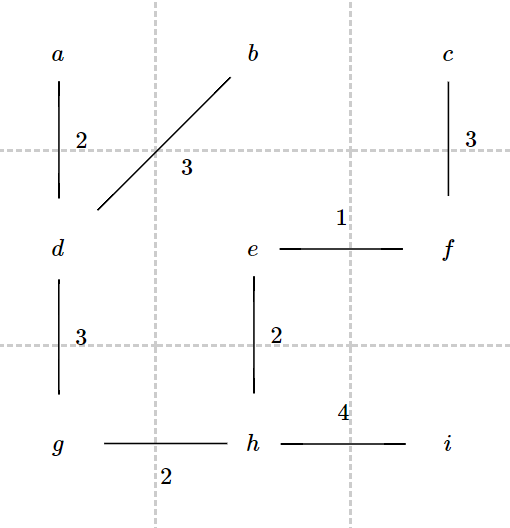
\includegraphics{graph_1}

\pagebreak
\subsection*{c)}

	For this graph yes. The selection of edges might change in terms of their order, but overall will be the same. 
	Both Prim's and Kruskal's algorithms give the same minimum spanning tree (MST).
	In general, it might not be the case: \\
	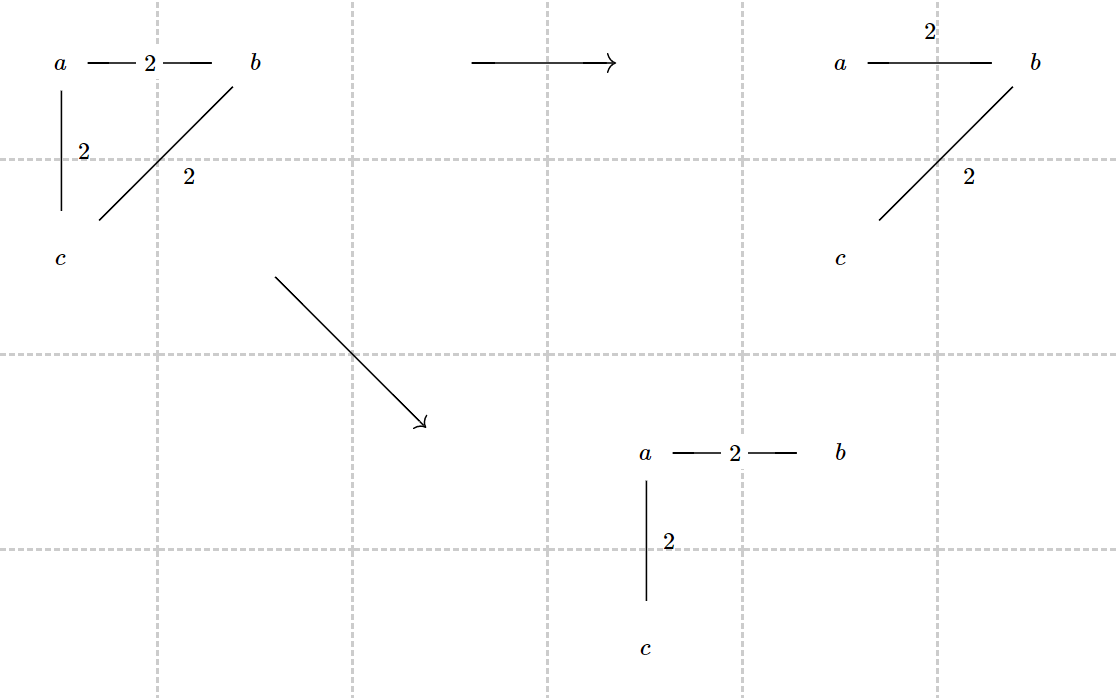
\includegraphics[scale=0.7]{graph_2}
	\\
	Above, there are more than 1 possible MST's.
	
\subsection*{d)}
	
	If we add the minimum weight edge to the hypothetical MST that does not contain it, there will be a cycle. To eliminate the cycle, we eliminate another edge which
	will be of larger weight. This will create a contradiction with the definition of MST. Therefore, MST always contains the minimum weight edge.

\section*{Answer 2}

	There is a correspondance between the two graphs. \\
	a - n 	\\
	b - q \\
 	c - o 	\\
	d - r  \\
	e - m 	\\
	f - p \\


\section*{Answer 3}

\subsection*{a)}

	vertices : 7 \\
	edges : 6 \\
	height : 3 \\

\subsection*{b)}

	postorder : q - s - u - v - t - r - p \\
	preorder  : p - q - r - s - t - u - v \\
	inorder    : q - p - s - r - u - t - v \\

\subsection*{c)}

	Yes. Because, every node has 2 or 0 children.

\subsection*{d)}

	No. Because, q has no child but r has. The order (from left to right) in inserting children is not obeyed.

\subsection*{e)}

	No, because of p. height(r) - height(q) > 1.

\subsection*{f)}

	No. (u:23) is in the right subtree of (r:24) but (u:23) < (r:24) which violates binary search tree property.

\subsection*{g)}

	A full binary does not have a vertex with a single child. Therefore, in each level except 0, there will be two vertices with a common parent. 
	There will be 6 levels in a binary tree of height 5. In total, $ 1 + 5 \cdot 2 = 11 $.












\end{document}